\chapter{Introduction a EMMA}
\label{ch:introduction}
% (cf loi de \cite{moore1965cramming}). 
%\cite{THOMPSON200620}

Les échelles de temps sont radicalement opposées entre la cosmologie qui considère les temps les plus long de l'univers et les progrès informatiques qui vont a une vitesse exponentielle.
Du fait de l'avancée rapide des moyens de calculs, les simulations numérique sont des produits possédant une valeur se dépréciant rapidement et doivent être considérées comme éphémère.

Nous avons vu dans la partie précédente qu'elles étaient les principales physiques à l’œuvre durant l'époque de réionisation.
L'objectif de cette partie est d'expliquer comment ces physiques sont modélisées et quelles sont le contraintes sur leurs  implémentations.

%Comment modéliser la reionization?

\section{Aperçu des différents modèles numériques}

Un code de simulation cosmologique a pour vocation principale de suivre l'évolution de différents "fluides", comme la matière noire, la gaz, les étoiles et la radiation (et parfois le champs magnétique).
Ces fluides sont de natures différentes et il n'y a pas de méthode unique permettant de suivre de manière optimale ces différentes physiques.
On distinguera principalement deux catégories de fluides: les collisionnels et les non-collisionnels.

\paragraph{La physique non-collisionnelle} concerne les phénomènes qui n'interagissent pas par collision.
Dans notre cas, il s'agit principalement la matière noire et les étoiles. 

\paragraph{La physique collisionnelle} concerne principalement le gaz.

Il existe conceptuellement deux principales façons de suivre un fluide dans l'espace.
%Ces deux approches sont dites \emph{Eulérienne} ou \emph{Lagrangienne}.
En lien direct avec ces deux familles de représentations physique, il existe deux principales familles de codes cosmologique% : les codes \ac{SPH} et les codes \ac{AMR}.

\paragraph{Représentation Lagrangienne : } 
consiste à se placer au point de vue du fluide.
Une série d'éléments de fluide de masse fixe pouvant se déplacer et/ou se dilater dans l'espace sera considérée.
Les codes utilisant ce type de représentation seront généralement associés avec une gestion de la physique sous forme de \emph{particules}.
Ces codes seront dit \ac{SPH}.

%\paragraph{\ac{SPH} : } représente le gaz sous forme de particule de masse constante mais de taille variable.
%Notion d'arbre -> KDtree

\paragraph{Représentation Eulérienne : } 
consiste a se placer au point de vue de l'espace.
On considère un élément d'espace et le bilan de matière entrant et sortant de chacune de ses interfaces.
On associera généralement les codes utilisant ce type de représentation avec une gestion de la physique sous forme de \emph{grille}.
Si la grille est de résolution variable on parlera de grille \ac{AMR}.

%\paragraph{Code sur grille} : représente l'espace sous forme de cellules organisées sur une grille. 
%Notion d'arbre -> arbre AMR
%La représentation Lagrangienne la plus populaire (dans le domaine des simulations cosmologiques) est sans doute le \emph{Smouth Particle Hydrodynamics (SPH) }
%Les volumes cosmologiques étant généralement cubique, les éléments de grille le sont généralement aussi.
%historique
%avantage inconvénient AMR vs SPH
%introduction de la grille et de la méthode AMR

Un même code peux utiliser conjointement plusieurs des concepts qui viennent d'être introduits.
Dans le cas présent, EMMA utilise une représentation Lagrangienne pour simuler la physique non collisionnelle de la matière noire et des étoiles, et une représentation Eulérienne pour simuler le gaz et la radiation.

\section{Gestion de la grille}
\label{sec_gestion_grille}
%(nécessaire d'être positionné ici car la structure en arbre conditionne plusieur choix par la suite)

Un des concepts le plus central de EMMA est sa grille adaptative.
Tout les solveurs sont basés dessus et sa structure conditionne un certain nombre de choix par la suite.
C'est pourquoi nous allons la développer ici, avant de détailler la gestion de la physique. 

Avant d'aborder le concept de grille adaptative faisons un léger détour par l'exemple d'une grille fixe et régulière.
Dans le cas des simulations sur grille fixe, les données sont réparties en mémoire de façon ordonnée.
Dans un espace en 3D, on accédera à une cellule contenant le point de coordonnées normées $(x,y,z)$ sur une grille de $N_x*N_y*N_z$ cellules, a l'aide de son identifiant Id dans le tableau en mémoire.

\begin{equation}
Id = i + j*N_x + k * N_x*N_y
\end{equation}
avec :
\begin{equation}
\begin{cases}
i=\lfloor x \rfloor *N_x \\
j=\lfloor y \rfloor*N_y \\
j=\lfloor z \rfloor*N_z \\
\end{cases}
\end{equation}
ou $\lfloor a \rfloor$ représente la partie entière de $a$.

Nous voyons ici que l'organisation en mémoire et la recherche de voisin sont relativement simple à gérer.
Les vecteurs sont alloués de manière statique et la recherche de voisin est basée sur un jeu d'indice relativement simple.
Les choses sont plus complexes dans le cas d'une grille adaptative.
Étant amenée à évoluer, il faut introduire des mécanismes permettant de construire ou détruire certaines parties de la grille de façons dynamique.
Ces mécanismes vont totalement changer l'organisation de la grille.

Un exemple de grille \ac{AMR} générée par EMMA est présenté sur la figure \ref{fig:AMR}).
Un fonction de critères prédéfinis par l'utilisateur la résolution de la grille peut être arbitrairement augmentée localement.
L'avantage de ce type de grille est d'économiser des ressoucres de calcul par rapport au cas d'une grille fixe, ou il faudrait beaucoup plus de cellules pour obtenir une résolution équivalente.

\begin{figure}[bth]
        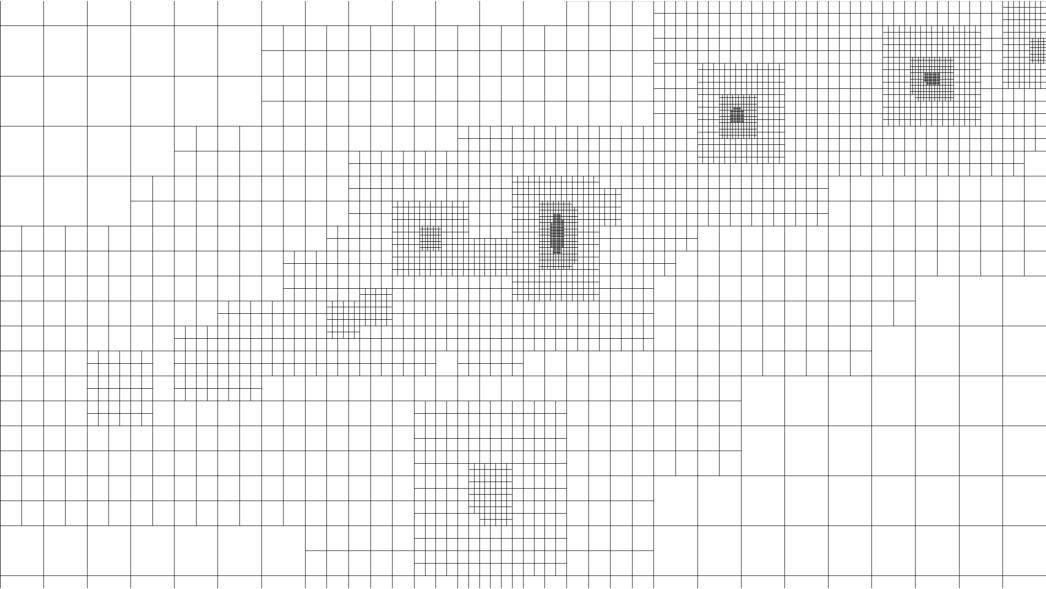
\includegraphics[width=.95\linewidth]{img/02/AMR.pdf} 
        \caption{Exemple de grille \ac{AMR} générée par EMMA. 
        La  résolution de la grille est augmentée arbitrairement dans les régions d'intérêts.
}
 		\label{fig:AMR}
\end{figure}



\subsubsection{Octree}

Il existe deux grands groupe de maille adaptative.
Le premier groupe utilise une séries de grilles fixes imbriquées. %TODO ref
Chaques région raffinée sera une grille fixe de résolution plus importante spatiallement liée a une grille de base.
Chaque nouvelle grille aura une résolution double par rapport a la précédente.
Il est possible d'ajouter autant de niveaux que voulu.

Le second est le groupe qu'utilise EMMA : fully threated tree description \citep{khokhlov_fully_1998-1}.
La base de cette représentation est de considérer que chaque cellule est associée à une grille fixe de taille 2x2x2 que l'on nommera un OCT , car décomposé en 8 cellules.
%sous parties qui sont elles même des cellules.
Et récursivement, chacune de ces cellules peuvent à leurs tour être divisée et  associée à un OCT.
Il en résultera un arbre nommé Octree, représenté sur la figure \ref{fig:octree}.

\begin{figure}[bth]
        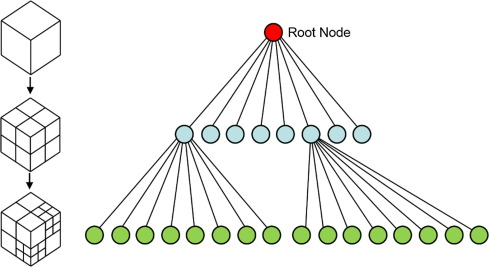
\includegraphics[width=.95\linewidth]{img/02/octree.jpg} 
        \caption{Représentation d'une grille AMR a gauche, et de son octree associé a droite. 
        Image extraite de \cite{SU201659}
     	\label{fig:octree}
}
\end{figure}

%TODO introduire construction de la grille et grille coarse
Pour créer une telle grille, il faudra d'abord créer un OCT, et le forcer à raffiner jusqu'à un niveau défini, ce niveau de base sera appelé par la suite niveau coarse.
Il en résultera une grille régulière qui ne pourra pas être dé-raffinée.

\subsubsection{La structure OCT}
%et liste chainée

Il existe une bimodalité entre la représentation de la grille en mémoire et la représentation de l'espace physique.
Comme la grille est amenée à évoluer, il n'y a plus une position unique en mémoire associée à une position dans l'espace.
De plus, le nombre d'éléments de la grille change au cours du temps.
Il faut donc conserver à la fois l'information de la position dans l'espace physique et dans l'espace mémoire.

En principe, on allouera une certaine quantité d'OCT en mémoire qui constituerons une réserve.
On viendra ensuite piocher dans cette réserve pour ajouter des éléments à la grille.
Les OCT de la grille seront organisés sous forme de liste chainées, il est donc nécessaire d'avoir l'information de la position de l'OCT précédent et de l'OCT suivant en mémoire.

Pour créer un lien entre elle, il est nécessaire de stocker l'information de voisinage.
L'information spatiale est aussi contenue dans les OCT, ceux ci disposent de  2*D pointeurs vers les cellules voisine.
Un OCT est également composé d'un tableau de huit cellules filles, ainsi que d'un pointeur vers sa cellule mère.
Un OCT qui n'a pas de cellule mère est appelé OCT racine, en pratique il n'y en a qu'un seul, de niveau 0, et il représente l'ensemble de l'espace de la grille..
La génération de conditions périodique (généralement utilisées en cosmologies) se fait de manière naturelle en faisant pointer tout les voisins de l'OCT racine vers lui même.
La structure minimal d'un OCT de EMMA est présenté sur le listing \ref{lst:oct}.

\begin{lstlisting}[float=bth,language=C,frame=tb,caption={La structure OCT de EMMA},label=lst:oct]
struct OCT{
  struct CELL cell[8]; // les 8 cellules de l'oct
  struct CELL *nei[6]; // pointeurs sur les cellule voisines
  struct CELL *parent; // cellule mere
  struct OCT *next;    // oct suivant dans la liste chainee
  struct OCT *prev;    // oct precedent dans la liste chainee
  int level;           // niveau de l'oct
};
\end{lstlisting}

\subsubsection{La structure CELL}

Les cellules contiennent l'information physique (densité, pression, température, etc...).
Chaque cellule peut, sous certaine condition, être subdivisée en un OCT pour augmenter la résolution localement.
L'information de la position de la cellule dans l'OCT parent est contenue dans son identifiant (allant de 0 à 7).
Une CELL qui n'a pas d'OCT enfant est dite cellule feuille.
La structure minimal d'une CELL de EMMA est présenté sur le listing \ref{lst:cell}.

\begin{lstlisting}[float=bth,language=C,frame=tb,caption={La structure CELL de EMMA},label=lst:cell]
struct CELL{
  int id;            // permet de determiner la position de la cellule dans l'oct
  struct OCT *parent // l'oct pere de la cellule
  struct OCT *child; // si child est different de NULL alors la cellule est raffinee et child point vers l'oct enfant
  struct PHYSIC *data; // pointeur vers la partie physique
};
\end{lstlisting}

\subsubsection{Gestion du raffinement}
\label{sec:raffinement}
%différentes condition de raffinement.\\
%sur la matière noire\\
%semi Lagrangienne\\
%sur le gradient d'ionization\\
%sur le gradient de densité (shock)\\

Il est possible de définir arbitrairement une condition de raffinement en fonction de la physique que l'on cherche a étudier.
Par exemple, dans des tests unitaires de type sphère de Stömgren (cf \ref{sec:stromgren}) ou explosion de Sedov (cf \ref{sec:sedov}), on marquera les cellules qui sont soumises à un gradient d'ionisation ou de densité supérieur à un certain seuil.
Dans le cas de simulations cosmologique, on utilisera généralement une condition dite semi-Lagrangienne.
C'est a dire qu'une cellule sera marquée comme "a raffinée" si la masse de matière noire (ou de gaz) qu'elle contient est supérieur a huit fois la masse de matière noire (ou de gaz) moyenne d'une cellule de ce niveau.

En pratique, le raffinement se fera en trois temps:

\begin{itemize}
\item Dans un premier temps le code va passer en revue toutes les cellules d'un niveau, et les marquer comme "à raffiner" si une première condition physique est respectée.

\item Une fois tout le niveau passé en revue, le code va ensuite faire une série de $N_{buffer}$ passages sur tout le niveau en marquant à chaque fois toues les cellules voisine des cellules précédemment marquées.
Cette série de passage a pour but d’élargir la zone de raffinement et ainsi permettre une transition douce entre les niveaux.
Cette zone de $N_{buffer}$ cellules autour des zones soumises à la condition physique de raffinement sera appelée le "buffer de raffinement".

\item Une fois les cellules respectant ces deux conditions marquées, le raffinement est effectué.
\end{itemize}

%En pratique le raffinement d'une cellule se fera en lui associant un OCT.
%*child pointera alors vers le dernier OCT libre de la liste chaînée.

%le deraffinement
On remarquera que la condition de raffinement ne prends pas en compte le fait qu'une cellule soit déjà raffinée ou non.
Si une cellule est raffinée, mais qu'elle n'est pas marquée comme "a raffinée" elle sera donc dé-raffinée.

\subsubsection{Opérateurs de changement de grilles} \label{Opérateurs de changement de grilles}

Les opérations de raffinement/dé-raffinement font intervenir des opérateurs de changement de grille.
Le changement de résolution peut avoir lieu dans les deux sens :

\begin{itemize}
\item La \emph{restriction} consiste à dégrader la grille en résolution. 
La restriction la plus directe consiste à moyenner les cellules à dégrader. 
Par exemple, sur une grille à deux dimensions, pour diviser la résolution par deux, quatre cellules de la grille de départ devront être moyennées pour obtenir une nouvelle cellule de la grille à base résolution.

\item La \emph{prolongation} consiste à augmenter la résolution d'une grille, la prolongation la plus directe consiste à injecter les valeurs de l'ancienne grille dans un certain nombre de cellules de la nouvelle grille. (fig \ref{Opérateurs de changement de grille})
\end{itemize}

\begin{figure}[htbp]
\begin{center}
\subfloat[Restriction]{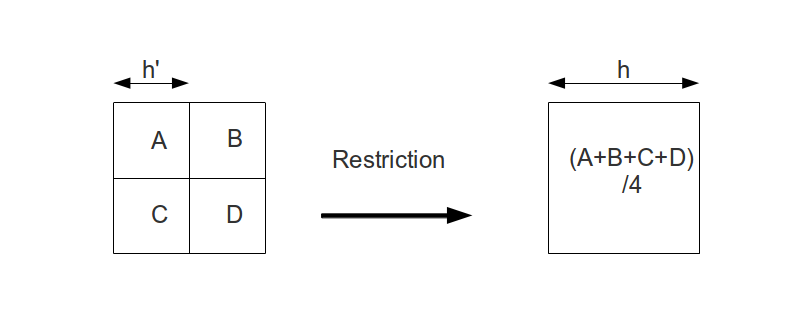
\includegraphics[width=.45\linewidth]{img/02/Restriction.png}}
\subfloat[Prolongation]{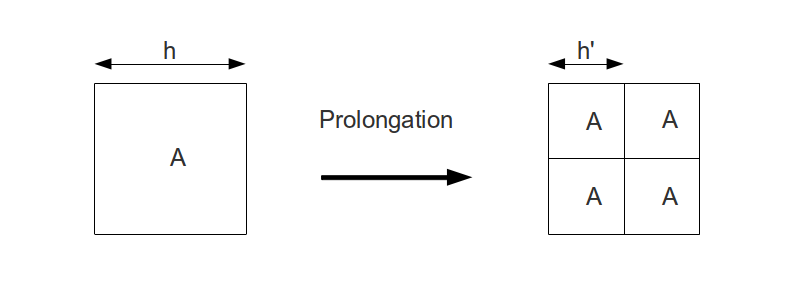
\includegraphics[width=.45\linewidth]{img/02/Prolongation.png}}\\
\subfloat[Niveau L  ]{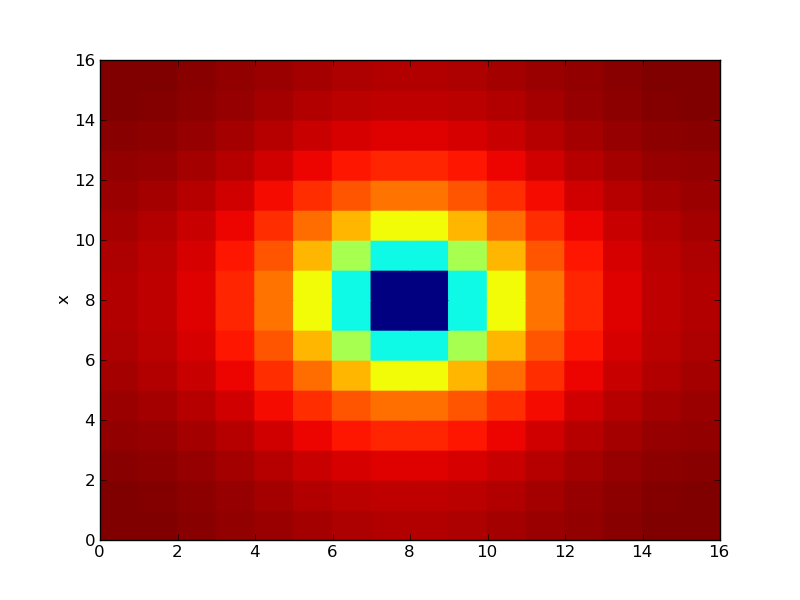
\includegraphics[width=.45\linewidth]{img/02/0090.png} \label{Opérateurs de changement de grille d}}
\subfloat[Niveau L+1]{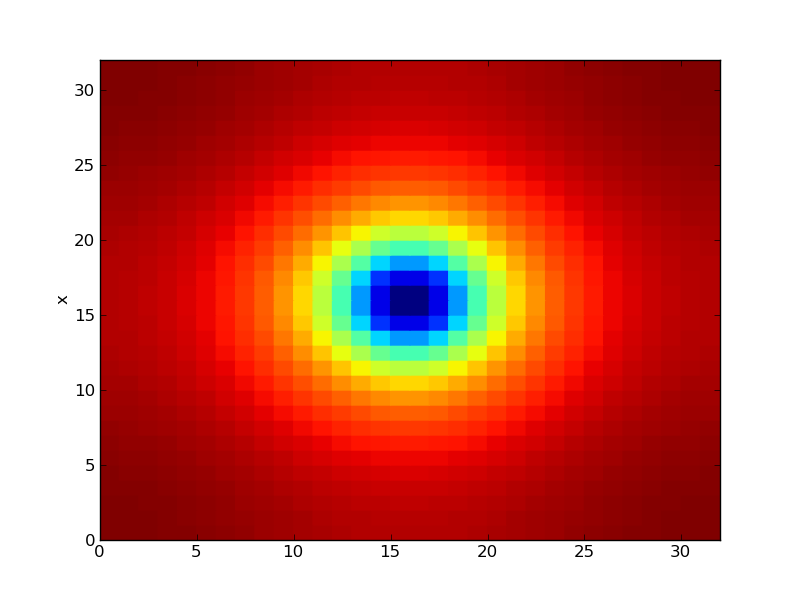
\includegraphics[width=.45\linewidth]{img/02/0088.png} \label{Opérateurs de changement de grille c}}
\caption{Opérateurs de changement de grille. 
Ils permettent de changer la résolution de la grille. 
Un exemple de restriction consiste à moyenner une valeur de plusieurs cellules, la prolongation associée consiste en une injection directe d'une valeur dans plusieurs cellules.
\label{Opérateurs de changement de grille}}
\end{center}
\end{figure}

%La prolongation et la restriction sont des opérateurs aisément parallélisables. Chaque cellule (ou paquet de huit cellules) est indépendante des autres et il est possible de ne changer la résolution que d'une partie de la grille sans en affecter le reste.

%Il existe principalement deux conditions sur les opérateurs de changement de grille. 
%La première impose une certaine réciprocité entre eux, les opérateurs doivent être adjoints: il est nécessaire qu'après une prolongation, suivie d'une restriction la grille d'arrivée soit la même que la grille de départ. 
%L'inverse n'est pas nécessairement vrai: après une restriction, de l'information est perdue et aucune prolongation ne pourra la recomposer.
%La seconde condition concerne la precision des opérateurs, il est nécessaire que la somme des ordres des opérations soit supérieure à l'ordre de l'équation à résoudre. 
%Ici, la restriction est d'ordre trois, la prolongation d'ordre un et le Laplacien d'ordre deux, cette condition est vérifiée.


\subsection{Recherche de voisin}
Nous verrons par la suite que l'état d'une cellule dépend des états des cellules qui l'entoure.
La recherche de voisins sera donc une étape importante dans la gestion de la grille.

La recherche de voisin se fera suivant ces étapes:

\begin{itemize}
\item en fonction de l'ID de la cellule, déterminer si la voisine est dans le même OCT parent.

\item
\begin{itemize}
\item Si c'est le cas, accéder a l'oct parent et a l'aide de l'indice du tableau de cellule, retrouver le voisin en question.
\item Si ce n'est pas le cas, accéder a la cellule mère de l'oct père et rechercher l'oct voisin
\end{itemize}

\end{itemize}

\subsection{Gestion de l'expansion}
\label{sec:supercomobil}

Nous avons vu dans l'introduction a la physique de la reionisationque l'énergie noire représente la majore partie du contenu de l'univers (cf \ref{sec:dark_egy}) .
Nous allons voir dans cette partie comme cette composante est traité numériquement.
Bien que nous sachions absolument pas ce que peux être physiquement l'énergie noire, nous en observons les effets : l'Univers est en expansion accélérée.
Le solveur gérant l'énergie noire n'est pas a proprement parler un solveur numérique, mais plutôt d'un système d'unité. % servant a normaliser la physique.
Il consiste a normaliser les grandeurs par une variable fonction du facteur d'expansion.

L'intégration de la cosmologie, régissant le lien en le temps et le facteur d'expansion sera réalisé une fois au moment de l'initialisation du code (cf Eq. \ref{eq:scale_t}).
Il en résultera une table, conservée en mémoire pendant toute l'exécution.
Le facteur d'expansion sera alors interpoler dans cette table ne fonction de l'avancement de la simulation.% (cf partie calcul du pas de temps) %TODO ref

Il existe deux possibilités pour modéliser l'expansion de l'univers à l'aide d'une grille.
La première consiste a considérer un élément de volume $dx$ de taille fixe, et au fur et a mesure que l'univers grandis, à y ajouter des éléments.
Le problème et que le coût numérique de la simulation croit, entre autre, avec le nombre d'éléments que l'on considère.
La seconde possibilité est de faire varier la taille des éléments de calcul avec le facteur d'expansion.
On appellera les longueurs ainsi exprimées des longueurs comobile.

\begin{equation}
r=a r'
\end{equation}

ou $r$ représente une longueur en unités physique et $r'$ en unités comobile.
Ainsi un cube de 10 Mpc physique de coté, pris aujourd'hui, aura une taille de 10 Mpc comobile (cMpc) aujourd'hui, mais aussi a redshift z=9 ou sa taille physique ne sera plus que de de 1Mpc physique.
De plus, il est généralement pratique de normaliser les grandeurs que l'on considère. 

\begin{equation}
r'=\tilde{r}r*
\end{equation}
ou $\tilde{r}$ est la longueur normalisée et $r*$ le facteur de normalisation.

La généralisation de ce principe a d'autre unités que la longueur est appeler système d'unités supercomobiles.
\citep{martel_convenient_1998}

\begin{table}[htbp]
\begin{center}
\begin{tabular}{r l} \hline 
Longueur: & $\tilde{r}=\frac{r}{ar_*}$ \\ \hline 
Densité de matière: & $\tilde{\rho}=\frac{\rho a^3}{\rho_*}$ \\ \hline 
Vitesse: & $ \tilde{v}=\frac{av}{v_*}$ \\ \hline 
Pas de temps: & $\tilde{dt}=\frac{dt}{a^2t_*}$\\ \hline 
Densité d’énergie potentielle: & $\tilde{\Phi}=\frac{a^2 \Phi}{\Phi_*}$\\ \hline 
Pression: & $\tilde{p}=\frac{a^5 p}{p_*}$\\ \hline 
Densité d’énergie cinétique: & $\tilde{\epsilon}=\frac{a^2 \epsilon}{\epsilon_*}$\\ \hline 
Densité D’éléments: & $\tilde{N}=a^3 N r_*^3$\\ \hline 
Flux: & $\tilde{F}=a^4 r_*^2 t_* F$\\ \hline 
\end{tabular} 
\end{center}
\caption{Passage du système d'unités physique vers le système d'unité supercomobile} 
\end{table}

\begin{table}[htbp]
\begin{center}
\begin{tabular}{r l} \hline 
Longueur  & $r_*=L$\\ \hline 
Densité & $\rho_* = \bar{\rho} = \frac{3H_0^2 \Omega_m}{8\pi G}$\\ \hline 
Temps & $t_* = \frac{2}{H_0 \sqrt{\Omega_m}}$\\ \hline 
Vitesse & $v_* = \frac{r_*}{t_*}$\\ \hline 
Potentiel & $\Phi_* = \frac{r_*^2}{t_*^2} = v_*^2$\\ \hline 
Pression & $p_* = \frac{\rho_* r_*^2}{t_*^2} = \rho_* v_*^2$\\ \hline 
Énergie & $\epsilon_* = \frac{p_*}{\rho_*} = v_*^2$\\ \hline 
\end{tabular} 
\end{center}

\caption{Facteurs de normalisation des différents grandeurs physique} 
\end{table}

\subsection{Gestion du pas de temps}
%TODO 


\begin{equation}
\frac{\delta a (\Delta t) } {a} < \epsilon
\end{equation}


\chapter{Les principaux solveurs physique}

Nous allons voir dans cette partie que plus une physique représente une part importante du contenu de l'Univers plus elle est simple et rapide a simuler.
Nous nous intéresserons à trois solveurs distincts:
\begin{itemize}
\item de matière noire
\item du gaz
\item de la radiation
\end{itemize}
Et ce, dans un ordre décroissant d'importance, relativement a la quantité d'énergie totale.

%%%%%%%%%%%%%%%%%%%%%%%%%%%%%%%%%%%%%%%%%%%%%%%%%%%%%%%%%%%%%%%%%%%%%%%%%%%%%%%%%%%%%%%%%%%%%%%%%%%%%%%%%%%%%%%%%%%%%%%%%%%%%%%%%%%%%%%%%%%%%%%%
\section{Matière noire}
\label{sec:solverDM}
La matière noire, dispose de propriétés de fluide non collisionelle, et se prête particulièrement bien à la représentation Lagrangienne, et donc a une simulation sous forme de particule.
Pour la simuler, on utilisera le principe des code Ncorp., c'est à dire qu'on utilisera un champs de particules massive interagissante par gravitation.
Il existe différentes techniques pour suivre l'évolution d'un tel système.
Toutes sont basées sur le même principe.
Les particules sont placée suivant une certaine condition initiale.
Et on cherche a connaitre la force gravitationnelle à laquelle chaque particule est soumise, dans le but de calculer son déplacement

\subsection{Génération des conditions initiales}
\label{sec:IC}
Nous avons vu (cf \ref{sec:CMB}) que le \ac{CMB} nous donne de l'information sur l'état de la distribution de matière dans l'univers très tôt dans son histoire.
Il est possible de déterminer le spectre de puissance des fluctuations de densité de l'univers primitif a partir du \ac{CMB}.
Le principe de la génération des condition initiales est d'utiliser ce spectre de puissance pour générer des surdensité représentant statistiquement ces fluctuations.

Pour se faire on va générer une grille régulière sur laquelle on placera une particule au centre de chaque cellule.
Dans ce cas la densité est homogène.
On va alors perturber la position des particules de manière à respecter les fluctuations statistique observées dans le CMB.
Pour ce faire, il faut générer un bruit aléatoire Gaussien.
%Tout les générateurs de condition initiales que j'ai pu rencontrer utilise une SEED aléatoire, dans le but de générer ce bruit aléatoire.
On convoluera ensuite ce bruit avec le spectre de puissance que l'on cherche a reproduire.
Et on appliquera les déplacement obtenus au particules.
Cette approximation n'est valable que dans le cas des petites perturbations, tant que l'on reste dans le régime linéaire et s'appelle l’approximation de Zeldovitch (eg \cite{2014MNRAS.439.3630W}).
L’approximation de Zeldovitch est capable de prédire analytiquement la distribution de la matière à très grandes échelles.
Mais plus l'on cherche à étudier des petites échelles, plus on sort vite du domaine de précision acceptable.
C'est pourquoi il est nécessaire d'avoir recourt au simulations numériques.

Nous voyons ici que le spectre est limité des deux cotés.
D'un coté l'information des grandes échelles est tronquée par la taille de la boite considéré.
Il n'est pas possible d'avoir de l’information sur des longueurs d'onde du spectre plus grande que cette taille limite.
De l'autre coté, les petites échelles sont tronquées par la limite de résolution.
Le spectre est troqué au niveau de la longueur d'onde correspondant à la résolution de la grille.
Cette perte d'information sur les hautes fréquences peux être problématique dans le cas où la résolution est adaptative.
Dans le cas de l'\ac{AMR} par exemple il peux paraître difficile d'autoriser un nombre élevé de niveau de raffinement puisque les niveaux nouvellement créer ne disposerons pas de l'information des conditions initiales.

%En pratique j'ai principalement utilisé MUSIC et GRAPHIC %TODO ref.

%méthode
%gaussian random noise
%théorie des perturbation linéaire
%lien avec le spectre de puissance
%MUSIC et GRAPHIC
%limite la résolution min et max (min en masse et max en espace)


%une simulation est limité par sa taille et sa résolution -> ceci définit la plage d'échelle que l'on peut simuler
%
%principes de bases ennoncé dans Pen (1997) and Bertschinger (2001).
%
%    discrétisation de l'espace
%    placement des particules sur la grille
%    génération d'un bruit blanc
%    convolution avec un spectre de puissance connu (celui du CMB)

%
%\subsection{Théorie des perturbation linéaire}
%
%approximation de zeldovich
%perte de linéarité a un certain moment -> nécessité des simulation numériques

\subsection{Solveur de gravité}
\label{sec:gravity}

%Je vais plus détailler le solveur de gravité que les autres puisque c'est celui sur lequel j'ai le plus travaillé.
%Le sloveur que je connais le mieux.
%Fluide non collisionnel -> particule\\

A partir des condition initiales générées par un code dédié, on cherche ensuite à suivre dynamiquement l'évolution des particules.
Le but est d'obtenir la position des particules à chaque instant.
Pour cela, il faut leurs vitesses.
Pour cela, il faut leurs accélération.
Pour cela, il faut la force qui leur est appliquée.
Et dans certain cas, il faut le potentiel gravitationnel.
Ce système d'équation est appelé le système d'équation de Vlasov-Poisson :

\begin{equation}
\begin{cases}

\frac{d{x}_p}{dt} = { v}_p, \\
\frac{d{ v}_p}{dt} = -\nabla \phi , \\
\Delta \phi= 4\pi G \rho.

\end{cases}
\label{eq:Ncorps}
\end{equation}

Il existe plusieurs méthodes pour résoudre ce système.
Historiquement la première méthode était la méthode :
\paragraph{Particule-Particule : } c'est la méthode la plus directe pour calculer l'évolution d'un system Ncorpsl. 
Elle consiste, pour chaque particule, à sommer les contributions gravitationnelles de toutes les autres particules:
\begin{equation}
\vec{F}_i=-\sum_{j\neq i} G \frac{G m_i m_j(\vec{r}_i - \vec{r}_j) }{ |\vec{r}_i - \vec{r}_j |^3}
\end{equation}
Ce type de code dispose d'une très bonne précision mais la quantité de calculs évolue en ordre $O(N^2)$, ce qui fait que ce type de code est très coûteux.

Une évolution de cette méthode est la méthode :
\paragraph{Particule-tree : } elle consiste a regrouper les particules les plus lointaine de la particule courante en amas aillant une interaction gravitationnelle commune.
% (Barnes & Hut 1986) 
Cette approximation permet de limiter considérablement le nombre de calcul pour les interactions lointaine qui sont de toute façons faibles.



%On peux obtenir cette force soit par calcul direct, soit par dérivation du potentiel.
%
%\begin{equation}
%\vec{F}=-\Delta \Phi
%\end{equation}

La méthode qui nous intéresse ici consiste à utiliser le potentiel pour déterminer la force.
Le potentielle sera calculé sur une grille, cette méthode sera nommée :
\paragraph{Particule-Mesh : } on projette les particules sur une grille dans l'objectif d'obtenir  une grille de densité pour ensuite obtenir le potentiel en resolvant l'équation de Poisson.
%ENZO %code, Bryan & Norman 1998
%RAMSES
La méthode de projection des particules sur la grille n'est pas unique.
A l'ordre 0, il est possible de se contenter d'ajouter la masse de la particule dans la cellule a laquelle elle appartient.
Le résultat obtenu étant très bruité, on utilisera une méthode d'ordre supérieure appelée \ac{CIC}:
\paragraph{CIC} consiste à considérer une étendue spatiale aux particules et à pondérer la masse appliquée aux cellules par l'intersection de son volume et de celui de la cellule (voir Fig\,\ref{fig:CIC}).
On associe généralement une taille à la particule similaire a celle des cellule sur laquelle on la projette.
Dans le cas où l’étendue de la particule intersecte des cellules de différents niveaux on lui associera la taille de la plus grande cellule dans le but de lisser la transition entre les niveaux.

\begin{figure}[bth]
		\centering
        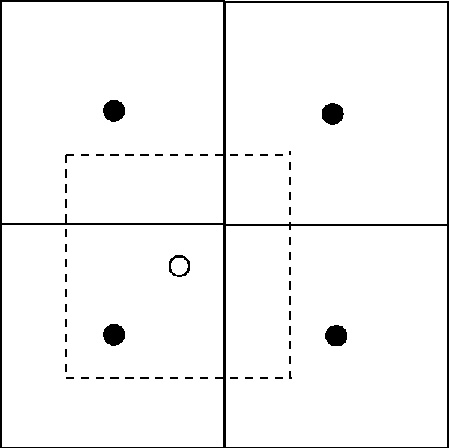
\includegraphics[width=.5\linewidth]{img/02/CIC.jpg} 
        \caption{Représentation en 2D du Cloud In Cell. 
        La masse d'une particule est répartie dans le cellules environnantes en lui associant une étendue spatiale.
        %http://homepage.univie.ac.at/franz.vesely/cp_tut/nol2h/new/c6sm_s4lr.html
}
 		\label{fig:CIC}
\end{figure}

Il existe des méthodes d'ordre supérieur avec des kernel plus complexe que le top-hat du \ac{CIC} comme par exemple des kernel en triangle ou en gaussienne.
%http://techfinder.stanford.edu/technology_detail.php?ID=30866
Une fois la grille de densité générée nous pouvons calculer le potentiel.

\subsubsection{l'équation de Poisson}

Connaissant la distribution de densité a un certain instant, il est possible de calculer le potentiel gravitationnel en résolvant l'équation de Poisson:

\begin{equation}
\Delta \Phi = S_{(\rho)}
\end{equation}

où :
\begin{equation}
S_{(\rho)} = 4 \pi G \rho
\end{equation}
dans le cas classique, et devient en système d'unité supercomobile (cf Sec. \ref{sec:supercomobil}):
\begin{equation}
S_{(\rho)} = 6 a \delta_{(\rho)}
\end{equation}
avec le contraste de densité: 
\begin{equation}
\delta_{(\rho)} = \rho / < \rho > - 1 
\end{equation}

L'objectif est donc d'intégrer deux fois la distribution de densité pour obtenir le potentiel gravitationnel:

\begin{equation}
\Delta \phi = S \longrightarrow \phi = \iint \Delta \phi = \iint S
\end{equation}

Pour cela, il existe principalement deux types de méthodes. 
La première est basée sur les transformées de Fourier. 
Cette méthode, très rapide, utilise le fait que dans l'espace de Fourier, une intégrale se résume à une division par un nombre d'onde. 
Déterminer le champ de potentiel revient à : 
\begin{itemize}
\item Effectuer la transformée de Fourier de la densité
\item Diviser par $k^2$
\item Effectuer la transformée de Fourier inverse
\end{itemize}

\begin{equation}
S_{(\vec{x})} \overset{FFT}{\longrightarrow}  S_{(\vec{k})} \times \frac{1}{k^2}  \overset{RFFT}{\longrightarrow}  \phi_{(\vec{x})}
\end{equation}

De par la nature des transformées de Fourier, le champ de densité doit être périodique pour que l'implémentation de cette technique ne se révèle pas trop complexe. 
Ce qui n'est pas un problème en simulation cosmologique, où les conditions de bords sont toujours périodiques mais est plus problématique lors de la simulation de structures isolées, telles les galaxies ou les amas de galaxies. 
De plus, les FFT nécessitent un échantillonnage régulier, ce qui implique que cette méthode est incompatible avec les méthodes AMR. 
%Et dernièrement, le passage dans l'espace des fréquences nécessite des conditions de types plans parallèles lors parallélisation, conditions incompatible avec la gestion de grille utilisé par les code AMR dont EMMA} fait partie. \\

Un autre type de méthode de résolution possible est une méthode itérative. 
Elle consiste à faire converger le potentiel à partir d'une condition initiale arbitraire. 
Ce type de méthode est plus lente que la méthode par FFT mais permet d'utiliser tout type de conditions de bords, d'être facilement parallélisable et surtout est compatible avec les méthodes basées sur des grilles adaptatives.
%Par la suite, c'est donc une méthode itérative et plus précisément une méthode \emph{Multigrille} qui à été développée.
%Le potentiel est alors dérivé pour obtenir la force ressentie dans chaque cellule. 
%Il est ensuite aisé de calculer l'accélération subie par les particules de chaque cellule, et par intégration temporelle, leurs nouvelles positions et vitesses.
Le principe de ces méthodes est d'introduire un terme temporel fictif et de rechercher un solution stationnaire a cette nouvelle équation.
Par analogie à l'équation de la chaleur par exemple, la densité correspond aux sources chaudes et le potentiel à la température, à $t=0$ les sources chaudes sont allumées et la chaleur se propage jusqu'a ce que le milieu ait atteint sa température d'équilibre. 
Ici, c'est donc la gravité qui se diffuse dans le milieu.

\begin{equation}
\dfrac{\partial \phi}{\partial t} = \Delta \Phi -S 
\end{equation}

\subsubsection{Méthode jacobi}

La méthode de Jacobi est la façon la plus simple de relaxer ce type d'équation, elle consiste à utiliser directement la forme discrète de l'équation de Poisson modifiée. 
L'équation à intégrer est:

\[ \dfrac{\phi^{t+1}_i - \phi^{t}_i}{\Delta t}  =  \Delta \phi_i^t - S_i \]

où, à 3 dimensions, le Laplacien s'exprime :

\[ \Delta \phi_i^t = \dfrac{\phi_{x+1,y,z}^t  + \phi_{x-1,y,z}^t + \phi_{x,y+1,z}^t  + \phi_{x,y-1,z}^t + \phi_{x,y,z+1}^t + \phi_{x,y,z-1}^t	- 6\phi_{x,y,z}^t}{\Delta x ^2} \]
		
Le principal avantage de cette méthode est qu'elle ne nécessite de connaître l'état du système qu'au temps $t$.
%Ainsi, chaque fils d'exécution parallèle (thread) est indépendant et n'a pas d'information à communiquer aux autres.

\subsubsection{Gauss Seidel}
Gauss-Seidel est une amélioration de Jacobi. 
Au lieu d'utiliser, à chaque pas de temps, les valeurs de la grille au niveau précédent, cette méthode consiste à toujours utiliser la valeur la plus à jour disponible. 
Une fois $\phi^{t+1}_0$ calculé à l'aide de $\phi^{t}_i$, la valeur de $\phi^{t+1}_1$ n'est pas calculée à l'aide de $\phi^{t}_0$ mais avec $\phi^{t+1}_0$. 
En utilisant toujours la valeur la mieux estimée, cette méthode accélère la convergence. 
L'intégration temporelle ne change pas, mais l'intégration spatiale devient: 

\[ \Delta \phi_i^t = \dfrac{\phi_{x+1,y,z}^t  + \phi_{x-1,y,z}^\mathbf{t+1} + \phi_{x,y+1,z}^t  + \phi_{x,y-1,z}^\mathbf{t+1} + \phi_{x,y,z+1}^t + \phi_{x,y,z-1}^\mathbf{t+1}	- 6\phi_{x,y,z}^t}{\Delta x ^2} \]

La parallélisation de cette méthode est plus compliquée que dans le cas de Jacobi. 
La détermination de la valeur de chaque cellule nécessite de connaître l'état le plus à jour de ses voisins et donc de faire passer de l'information entre les threads.
Cependant, une méthode nommée Gauss-Seidel Rouge-Noir permet une parallélisation sur multiprocesseurs en séparant l'espace en un damier de couleurs. 
Chaque processeur ne calcule alors qu'une seule couleur. 
Le premier processeur calcul par exemple les cases blanches de l'échiquier à partir de $\phi_i^t$, puis le second calcul le cases noires à partir des cases blanches déterminé par le premier.


\subsubsection{Sur-relaxation successive (SOR)}
La méthode de sur-relaxation successive consiste à appliquer un coefficient à la méthode de Gauss-Seidel (ou de Jacobi, en fonction de la méthode de dérivation spatiale) pour sur-estimer l'évolution de la convergence et ainsi l'accélérer. 
L'équation à intégrer devient:
\[ \phi^{t+1}_i = \phi^{t}_i + \omega  \Delta t \left (\Delta \phi_i^t -S^t_i \right )  \]
où $\omega \in \left] 0,2 \right [$ est le paramètre de sur-relaxation.
\begin{itemize}
\item lorsque $\omega <1$ La méthode est dite de sous relaxation.
\item lorsque $\omega =1$ La méthode devient celle de Gauss-Seidel.
\item lorsque $\omega >1$ La méthode est dite de sur relaxation.
\end{itemize}
Il existe des moyens analytiques pour déterminer la valeur optimale de $\omega$ mais très souvent cette valeur est déterminée empiriquement à partir d'une série de tests. 
$\omega = 1,2$ est très souvent utilisé.
%L'expression de cette méthode apparait généralement dans la litterature sous la forme:

\subsubsection{Condition d'arrêt}
Ces méthodes sont itérées jusqu'à ce qu'un certain critère convergence soit respecté. 
Le critère le plus couramment utilisé consiste à mesurer l'évolution de la convergence en comparant sa valeur au temps $t$ à celle au temps $t+1$.
\[ \phi^{t+1}_i - \phi^{t}_i < \epsilon \]
ou, de manière équivalente:
\[ \Delta \phi_i^t - S_i^t< \epsilon \]

Pour prendre en compte la possibilité que le potentiel ait convergé sur une partie du domaine seulement, et pour ne pas stopper le processus trop tôt, c'est le module de cette expression qui est considéré. 
De plus il est d'usage de normaliser ce module par la source que l'on considère.

\[\dfrac{ \sqrt{  \sum_i \left (  \Delta \phi_i^t \right )^2 - \left (S^t_i  \right )^2 } }{\sqrt{  \sum_i  \left (S^t_i  \right )^2 } } < \epsilon \]

A cette condition est ajouté un nombre d'itérations maximum fixe pour éviter les problèmes de boucles infinies lorsque le potentiel n'arrive pas à converger (oscillation autour d'une valeur d'équilibre par exemple).

\subsubsection{Multigrille}

La technique du multigrille a été développé pour améliorer la vitesse de convergence des méthodes itératives.
Elle consiste à travailler non pas sur la grandeur elle même, mais sur l'erreur effectuée dans l'estimation de cette grandeur.
 
Si l'équation à résoudre est de la forme : 
\[ \mathcal{L} u = f \]
Sa forme discrète est :
\[ \mathcal{L}_h u_h = f_h \]
si $\tilde{u_h}$ correspond à une estimation de la solution et $u_h$ à la solution exacte, l'erreur est alors la différence entre les deux : 
\[ v_h = u_h - \tilde{u_h}. \]
Le résidu est défini comme:
\[ d_h = \mathcal{L}_h \tilde{u_h} - f_h \]

Et en utilisant la linéarité de l'opérateur Laplacien:
%comme $\mathcal{L}_h$ est linéaire:
\[ \mathcal{L}_h u_h = \mathcal{L}_h (v_h + \tilde{u_h} ) = \mathcal{L}_h v_h +\mathcal{L}_h \tilde{u_h} \]
\[ f_h   = \mathcal{L}_h \tilde{u_h} - d_h\]
et finalement :
\[ \mathcal{L}_h v_h = -d_h \]

L'équation à résoudre est alors modifiée en considérant que l'inconnue n'est plus le potentiel mais l'erreur commise sur son estimation. Le terme source n'est plus la densité mais la densité moins son estimation grossière.\\

Le cycle consiste à lisser (relaxer quelques fois) le potentiel à pleine résolution, les petites échelles vont alors rapidement converger, puis à calculer l'erreur commise à ce stade. 
L'erreur est dégradée à plus basse résolution, elle ne contient alors que de l'information sur les basses fréquences de la grille de départ, les hautes fréquences de la grille à pleine résolution ont été supprimées par la dégradation. 
Cette perte d'information sur les hautes fréquences n'est pas problématique car les hautes fréquences ont déjà convergé l'erreur est donc petite (voir nulle) aux hautes fréquence et est maximale aux basses. 
Les hautes fréquences de cette nouvelle grille correspondent alors à des fréquences plus basses et donc plus difficiles à faire converger sur le grille globale. 
La solution exacte de l'équation de l'erreur est calculée par itération (relaxée jusqu'à convergence) à partir des résidus sur cette petite grille. 
Le potentiel précédemment estimé est alors corrigé de l'erreur exacte interpolée à pleine résolution en utilisant:
\[ \tilde{u}_h^{new} = \tilde{u_h} + v_h \]
Le potentiel corrigé est alors lissé par quelques dernières itérations.
Ce cycle peut être résumé ainsi:

\begin{tabular}{ll}
Lisser 		& 	$ \mathcal{L} u_h = f_h $\\
Calculer	&	$ d_h = \mathcal{L}_h \tilde{u_h} - f_h $\\
Restreindre	&	$ d_H = Rd_h$\\
Résoudre	&	$ \mathcal{L} v_H = -d_H $\\
Interpoler	&	$ v_h = Pv_H$\\
Corriger	&	$ \tilde{u}_h^{new} = \tilde{u_h} + v_h$\\
Lisser		&	$ \mathcal{L} u_h = f_h $
\end{tabular} 

A partir de la méthode deux grilles, rien n'empêche d'estimer l'erreur sur l'erreur par la même méthode, ce processus peut être utilisé récursivement pour générer tout un ensemble de sous grilles et ainsi accélérer encore la convergence.\\

L'algorithme devient alors:\\

MG(level, $u_h$, $f_h$)
\begin{itemize}	
\item 	si level = level min:
\item[]	\begin{tabular}{ll}
		Résoudre & $\mathcal{L} u_h = f_h $
		\end{tabular}
\item 	sinon:
\item[]	\begin{tabular}{ll}
		Lisser 		& 	$ \mathcal{L} u_h = f_h $\\
		Calculer	&	$ d_h = \mathcal{L}_h \tilde{u_h} - f_h $\\
		Restreindre	&	$ d_H = Rd_h$\\
		Appeler 	&	MG(level-1, $v_H$, $-d_H$) \\
		Interpoler	&	$ v_h = Pv_H$\\
		Corriger	&	$ \tilde{u}_h^{new} = \tilde{u_h} + v_h$\\
		Lisser		&	$ \mathcal{L} u_h = f_h $
		\end{tabular} 
\end{itemize}

Où la taille de la grille au niveau "level" est de $2^{3L}$ ( si $L=9$, la taille de la grille est de $512^3$ ). $h$ est le pas de la grille au niveau $L$ est $H = 2h$. 
Les opérateurs $P$ et $R$ sont les opérateurs de prolongation et de restriction explicité section \ref{Opérateurs de changement de grilles}.
Cet algorithme est représenté graphiquement sur la figure \ref{Description du V-cycle}.

\begin{figure}[htbp]
\begin{center}
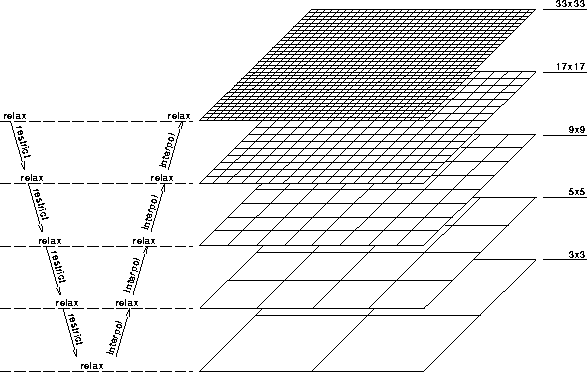
\includegraphics[scale=0.35]{img/02/multigrid.png}
\caption{\textbf{Vue des différents niveaux de grilles.} Image extraite de \href{http://MGNet.org}{MGNet.org} }
\label{Vue des différents niveaux de grilles}
\end{center}
\end{figure}	

\begin{figure}[htbp]
\begin{center}
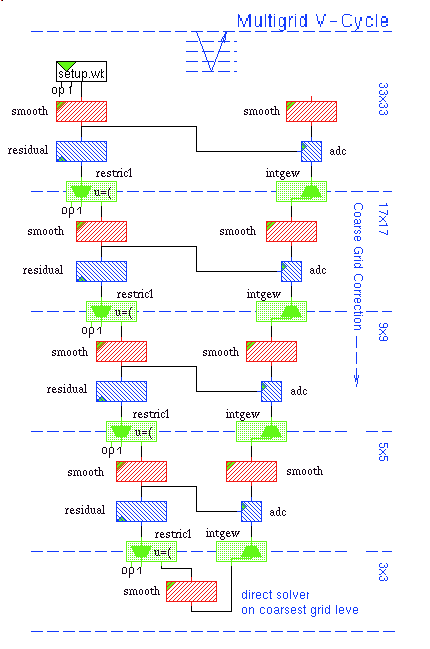
\includegraphics[scale=0.35]{img/02/Vcycle.png}
\caption{\textbf{Description du V-cycle.} Image extraite de \href{http://MGNet.org}{MGNet.org}}
\label{Description du V-cycle}
\end{center}
\end{figure}		

En jouant sur le nombre d'appels récursifs de la fonction, il est possible de créer différentes géométries de cycles. 
Un seul appel génère un cycle nommé cycle en V (fig. \ref{Description du V-cycle}), deux un cycle en W, etc... 

\subsection{Implémentation dans EMMA}
Dans EMMA, la potentiel est calculé par multigrille sur la grille coarse et utilise l'arbre \ac{AMR} pour gérer les sous-niveaux.
Sur les niveaux raffinés la relaxation est effectuée par Gauss Siedel rouge/noir.
La solution déterminée sur les niveaux grossiers est projetée sur les niveaux raffinés, la solution anticipée est deja proche de sa vraie valeur. 
Il en résulte une convergence rapide.

On prendra garde, lors de calcul en parallèle, à utiliser un niveau minimum de telle sorte que chaque processeur dispose au minimum d'un oct lors du calcul sur la grille grossière du multigrille.
%Dans le cas contraire, le calcul ne donnera pas le bon résultat.

\begin{equation}
L_{min} = 1 + ceil \left(\frac{log_2(N_{cpu})}{3}  \right) 
\end{equation}


\subsection{Liste chaînée de particule}
La gestion des particules dans EMMA utilise le principe de la liste chaînée déjà abordée pour les OCT. %TODO ref
A chaque cellule est associée  un pointeur vers une particule de tète.
Si ce pointeur est NULL, la cellule ne contient pas de particule.
Les particules entrant dans cette cellule seront ajoutées a la liste chaînée.
On prendra garde a gérer cette liste au moment du raffinement et du déraffinement des cellules.



\subsection{Le pas de temps}

Le pas de temps sera calculer de telle sorte a respecter la condition de Courant.
Une particule ne doit pas se déplacer de plus d'une fraction de case a chaque pas de temps.


%	    dtloc=0.1*SQRT(2.*M_PI/(3.*(curoct->cell[icell].gdata.d+1.)*aexp));
%\begin{equation}
%
%\end{equation}



%%%%%%%%%%%%%%%%%%%%%%%%%%%%%%%%%%%%%%%%%%%%%%%%%%%%%%%%%%%%%%%%%%%%%%%%%%%%%%%%%%%%%%%%%%%%%%%%%%%%%%%%%%%%%%%%%%%%%%%%%%%%%%%%%%%%%%%%%%%%%%%%

\clearpage
\section{Le solveur hydrodynamique et la physique baryonique}

%solveur hydro
%partie la plus intensive en calcul

Le solveur hydrodynamique est la partie du code sur laquelle j'ai le moins travaillé.
C'est aussi certainement l'une des plus complexe.
Dans un soucis de complétude, je vais tout de même en exposer les grandes lignes.
Mais cette partie sera moins étoffée que celles des autres solveurs numériques.

Comme nous l'avons vu plus tôt (cf \ref{sec:nucleosynthese_primordiale}), l'Univers est constitué d'une grande quantité d'hydrogène et d'hélium sous forme gazeuse.
Dans le cas de l'étude de l'\ac{EoR} la physique du gaz est centrale, car l'objectif est précisément de déterminer les propriétés physicochimiques de ce gaz, et leurs impacts sur la formation des galaxies.

Ici, le gaz est principalement soumis a deux forces : sa pression interne et la gravité.
La physique du gaz est régie par les equations d'Euler auto-gravitantes :

\begin{equation}
\begin{cases}

{ \frac{ \partial \rho }{ \partial t } + \nabla \cdot (\rho v) = 0}, \\
\\
{ \frac{ \partial }{ \partial t } (\rho v) + \nabla \cdot (\rho v \otimes v ) \nabla p = -\rho\nabla \phi }, \\
\\
{ \frac{ \partial e }{ \partial t } + \nabla \cdot [ \rho v (e+p/\rho) ] = -\rho v \cdot \nabla \phi },

\end{cases}
\end{equation}
\label{eq:hydro}

Ce set d'équations peut être réécris sous la forme:

\begin{equation}
U+F(U) = 0,
\end{equation}

avec:
\begin{equation}
U=
\begin{cases}
{ \rho}\\
{ u}\\
{ v}\\
{ w}\\
{ E}
\end{cases}
,
F(U)=
\begin{cases}
{ \rho u}\\
{ \rho u^2+p}\\
{ \rho uv}\\
{ \rho uw}\\
{ u(E+p)}
\end{cases}
\end{equation}

Pour suivre l'évolution de ce gaz nous allons le considérer comme parfait et monoatomique.
L’équation d'état du gaz sera donc:
\begin{equation}
p=\rho k T, 
\end{equation}
avec $k=1.38064852 \cdot 10^{-23} \left[ \mathrm{m^2 \cdot kg \cdot s^{-2} \cdot K^{-1}} \right] $ la constante de Boltzmann.


\subsection{Le problème de Riemann}
L'idée est de décomposer le domaine en cellules dans lesquelles les grandeurs seront localement constantes. (Piecewise constant approximation)
On utilisera ensuite les equations d'Euler pour résoudre localement le problème de Riemann a chaque interfaces de cellule.
Nous aurons donc accès aux flux de matière et d'énergie entre les cellules pour pouvoir calculer l'état suivant  

Le problème de Riemann consiste a considérer l’évolution d'un system d’équations différentielles à partir d'une condition initiale.
En aillant l’état d'un système régis par des equations différentielles un instant donné, qu'elle sera sont évolution?

\begin{itemize}
\item PDE
\item IC
\item BC
\end{itemize}

\subsection{La discrétisation du problème.}

Contrairement à la résolution de l’équation de Poisson, il n'est plus possible d'utiliser une discrétisation des dérivées à l'aide d'un différence finie centrée.
Nous allons rapidement voir pourquoi dans cette section.

Une différence finie centrée peut être décomposée en deux différence finies : 
\begin{equation}
\frac{d u}{dx} \approx \frac{u_{i+1}  + u_i}{\Delta x} 
\end{equation}

\begin{equation}
\frac{d u}{dx} \approx \frac{u_i  + u_{i+1}}{\Delta x} 
\end{equation}

Considérons que nous voulons résoudre l'équation :
\begin{equation}
\frac{du}{dt} + a\frac{du}{dx} = 0
\end{equation}

Dans le premier cas, la discrétisation pourra s'écrire : 
%la propagation d'une onde a la vitesse $a$ pourra être discrétisée en utilisant.

\begin{equation}
\frac{u_i^{t+1} + u_i^t }{\Delta t}   +a \frac{u_{i+1}^t  + u_i^t}{\Delta x} = 0
\end{equation}

\begin{equation}
u_i^{t+1}  = u_i^t +  c \left( u_{i+1}^t  + u_i^t \right) 
\end{equation}

ou : 

\begin{equation}
c= \frac{a \Delta t}{\Delta x},
\end{equation}
est le nombre de Courant

A l'aide d'une analyse de von-Neumann (cf \cite{toro1999riemann}), on montre que la stabilité de ce schéma dépend du signe de a, la vitesse de propagation de l'onde.

\begin{itemize}
\item si a est positif, ce schéma est conditionnellement stable (la condition étant que la condition de Courant soient respectée : $0<c<1$) .
Ce schema est appélé méthode UPWIND.

\item A l'inverse on montre que que dans le cas de la seconde différence finie, le schéma est inconditionnellement instable. 
Ce shema est appelée méthode DOWNWIND.
\end{itemize}

Seule la méthode upwind permet de suivre correctement la propagation d'onde.
Le problème est qu'a trois dimension, il est impossible de respecter cette condition pour un système quelconque.
% déterminer dans quelle direction se propage une onde quelconques.

De plus il a été montré que cette méthode n'est pas conservative, et qu'elle était incapable de suivre les chocs (fortes discontinuités)

\subsection{Méthode de Godunov}

Godunov  \cite{MR0119433} a répondu a ce problème.

methodes conservative

introduction aux volumes finis
consiste a estimer le flux aux interfaces des cellules.


%\subsection{discretisation}
\begin{equation}
 \frac{\partial U}{\partial t} + \nabla \cdot (F(U)) = S(U), 
\label{eq:rad_generale}
\end{equation}

avec $U$ le vecteur des quantité conservées, $F$ la fonction de flux, et $S$ le terme source. Pour la résolution du transport des photons (sans terme source), on retrouve :

\begin{equation}
\frac{ u^{t+1}_i - u^t_i }{\Delta t} + \frac{ F^t_{i+1/2} - F^t_{i-1/2} }{\Delta x} =0,
\label{eq:rad_solver}
\end{equation}

ou $F^t_{i+1/2}$ et $F^t_{i-1/2}$ sont les flux numérique intercellules, une estimations des flux physique.

$F^t_{i+1/2}$

\subsection{Méhtode HLL et HLLC }
La méthode de HLL Harten, Lax et van Leer 
recalculation des flux entre les cellules

\subsection{MUSCL}
Monotonic Upstream-Centered Scheme for Conservation Laws (van Leer, 1979)
Consiste a considerer une valeur dans la cellule, non plus constante mais variable.
Cette variation est interpolée linéairement
%En utilisant la méthode de pente.

\subsection{Minmod}



\subsection{Le pas de temps}

Le pas de temps respecte encore une fois la condition de courant.

\begin{equation}
\frac{dx * CFL }{3*(max(v) + c_s)}
\end{equation}

avec $cs = \gamma P/\rho$

%%%%%%%%%%%%%%%%%%%%%%%%%%%%%%%%%%%%%%%%%%%%%%%%%%%%%%%%%%%%%%%%%%%%%%%%%%%%%%%%%%%%%%%%%%%%%%%%%%%%%%%%%%%%%%%%%%%%%%%%%%%%%%%%%%%%%%%%%%%%%%%%

\clearpage
\section{Le solveur radiatif}
\label{sec:rad_solver}

Il existe deux grandes famille de code de transfert de rayonnement.
\begin{itemize}
\item La première famille utilise une représentation très physique de la lumière, et simule la radiation a l'aide de rayons se propageant dans l'espace.
CRASH \citep{2003MNRAS.345..379M}, C$^2$RAY\citep{2006NewA...11..374M}.
Ce type de code utilise une principe qui se rapproche physiquement de la vraie nature de la lumière.
Chaque source lance un certain nombre de groupe de photon, qui vont se propager et interagir avec le milieu.
Plus les sources sont nombreuses, plus le nombre de groupe de photons a suivre devient important, et plus le cout numérique l'est également.

\item La seconde, celle utilisée dans EMMA, repose sur le principe de considérer la lumière comme un fluide. \citep{gnedin_multi-dimensional_2001, aubert_radiative_2008}.
Ces méthodes dites méthodes aux moments utiliseront donc les même concepts que le solveur hydrodynamique, mais avec un système initial d'équations différentes. 
EMMA utilise une approximation du moment au premier ordre, son solveur repose sur l'\textit{approximation M1} \citep{levermore_relating_1984}.
Son principal avantage est que le coût numérique est indépendant du nombre de sources.
\end{itemize}

Ce solveur se déroule en deux temps.
Premièrement, il faut calculer la propagation du rayonnement, on appelles cette étape \textit{le transport} des photons.
Deuxièmement, il faut le couplage entre le rayonnement et le gaz, c'est a dire calculer l'impact \textit{chimie} du gaz.


\subsection{Les équations du transfert du rayonnement}
\begin{equation}
\frac{1}{c} \frac{\partial I_\nu}{\partial t} + \vec{n}\cdot \vec{\nabla} I_\nu = \eta_\nu - \kappa_\nu I_\nu 
\end{equation}
Avec: $I_\nu(\vec{x},\vec{n},t)$ l'intensité spécifique,
$\eta_\nu(\vec{x},\vec{n},t)$ la source de rayonnement,
le coefficient d'absorption $\kappa_\nu(\vec{x},\vec{n},t) = \sigma_\nu n_H$, 
$\sigma_\nu$ la section efficace de photo-ionisation de l'hydrogène neutre et $n_H$ la densité d'hydrogène neutre


\begin{equation}
\begin{cases}

\frac{ \partial N_\nu }{ \partial t } + \vec{\nabla} \cdot \vec{F}_\nu = -\kappa_\nu c  N_\nu + S_\nu,\\

\frac{ \partial \vec{F} }{ \partial t } + c^2 \vec{\nabla} P_\nu = -\kappa_\nu c \vec{F}_\nu ,

\end{cases}
\label{eq:densite_energie}
\end{equation}
Représentant respectivement les moments d'ordre 0 et 1 de $I_\nu$ avec:
$\vec{F}_\nu$ le flux radiatif, 
$P_\nu $ la pression radiative
et $S_\nu = \dot{N}_\nu^* + \dot{N}_\nu^{rec}$ le taux d’émission de photon due aux sources $\dot{N}_\nu^*$ et a la recombinaison $ \dot{N}_\nu^{rec}$


\subsection{Relation de fermeture et approximation M1}
La fermeture du système se fait par l’intermédiaire de l’équation d’état, avec $D$ le tenseur d’Eddington :

\begin{equation}
 P_\nu = D N\nu ,
\label{eq:fermeture}
\end{equation}

où D est approximé par le modèle M1 \citep{levermore_relating_1984}%,gonzalez2005} :

\begin{equation}
\begin{cases}

D = \frac{ 3\chi -1 }{2} \mathbb{1} + \frac{ 1 - \chi }{2} \vec{n} \otimes \vec{n} , \\
\\
\chi(\vec{f}_\nu) = \frac{ 3+4 |\vec{f}_\nu|^2 }{5+2\sqrt{4-3|\vec{f}_\nu|^2}} , \\
\\
\vec{f}_\nu = \frac{ \vec{F}_\nu }{c N\nu }  ,

\end{cases}
\label{eq:tenseur}
\end{equation}


\subsection{Pas de temps et vitesse de la lumière réduite}

Condition de Courant radiative : $ c \leq \Delta x / \Delta t $.
Le pas de temps est donc plusieurs ordres de grandeur plus petit que celui de l'hydrodynamique.

%Pour compenser cette 

Les simulation cosmologique utilise l'approximation Newtonienne: les processus entrant en jeux on des vitesses très inférieurs a celle de la lumière.
L'idée est de diminuer la vitesse de la lumière dans le code tout en restant dans le domaine de l'approximation newtonienne.
Cette idée est développée en détails dans la section %TODO ref



\subsection{La chimie}

La chimie fait le lien entre le solveur radiatif et le solveur hydrodynamique.
C'est a ce moment qu'est appliquée l'énergie apportée par la radiation au gaz.
gestion du refroidissement/ de la température/ énergie interne
Contrairement au transport, la chimie est non conservative.

Densité de photons
\begin{equation}
\frac{dN}{dt} = S - c \sigma_N n_H N + \left( \alpha_A(T)  - \alpha_B(T) \right) x^2n_0^2
\end{equation}

Flux de photons
\begin{equation}
\frac{dF}{dt} = - c \sigma_N n_H F
\end{equation}

État d'ionisation
\begin{equation}
\frac{dn_H}{dt} =  \left( \alpha_A(T)x^2  - \alpha_B(T)x (1-x) \right) n_0^2 - c \sigma_N n_HN
\end{equation}


Énergie interne
\begin{equation}
\frac{de}{dt} = c n_H \Sigma_E N - \Lambda_{(n_0,x,T)}
\end{equation}


Les taux de réaction chimique $\alpha_A(T)$, $\alpha_B(T)$ et $\beta_(T)$ sont repris de tables de \cite{theuns_p^3m-sph_1998}.
Les sections efficace d'interactions viennent de \cite{hui_equation_1997}.

Les processus chimique agissant sur des échelles de temps courtes par rapport au transport des photons, le pas de temps sera plusieurs ordres de grandeurs plus faible.
En pratique, a chaque pas de temps radiatif, on effectuera un sous-cyclage sur le pas de temps chimique.
Après chaque pas de temps chimique, la variation d’énergie est calculée. 
Si celle ci est supérieure a 10\%, le pas de temps est divisée par 2 et l'étape courante est recalculée. (cf \cite{rosdahl_ramsesrt_2013}) 

Étant donné que le processus chimique sont uniquement local (ils ne dépendent pas de l'état des cellules voisines) et que la quantité de calcul est relativement importante, le portage du solveur chimique sur GPU est très intéressant du point de vue accélération.


\subsection{Groupes de photons}
\label{sec:groupedephotons}

Il n'est pas possible avec la méthode au moment de considéré directement un spectre d'émission.
Le spectre doit être discrétisé, c'est a dire qu'il devra être découpé en un certain nombre de groupe, et chaque groupe disposera des caractéristique moyenne de sa portion du spectre.
Le problème est que chaque groupe de photon devient un fluide a simuler. 
L'augmentation du nombre de groupe devient vite coûteux en terme de temps de calculs.

%Les caratéristiques des photons\\

Nous aborderons la mise en place du multi longueur d'onde dans la section %TODO ref


